% IEEE conference paper: DSCMR and CLIP4CMR on Pascal Sentence.
% Compile with XeLaTeX (tested). On Overleaf: upload main.tex and fig_results.pdf,
% then set Menu > Compiler > XeLaTeX. The pdfLaTeX branch (vntex/T5) is untested.
\documentclass[conference]{IEEEtran}

\usepackage{iftex}
\ifPDFTeX
  \usepackage[utf8]{inputenc}
  \usepackage[T5,T1]{fontenc}
  \newcommand{\vn}[1]{{\fontencoding{T5}\selectfont #1}}
\else
  \usepackage{fontspec}
  \setmainfont{texgyretermes}[Extension=.otf, UprightFont=*-regular, BoldFont=*-bold,
    ItalicFont=*-italic, BoldItalicFont=*-bolditalic]
  \newcommand{\vn}[1]{#1}
\fi
\usepackage{amsmath}
\usepackage{graphicx}
\usepackage{booktabs}
\usepackage{url}

\newcommand{\Asem}{A\textsubscript{sem}}
\newcommand{\Ares}{A\textsubscript{res}}

\begin{document}

\title{Semantic Prototypes and Stronger Visual Features for Supervised Image--Text Retrieval: Revisiting DSCMR and CLIP4CMR on Pascal Sentence}

\author{
\IEEEauthorblockN{\vn{Vũ Quốc Đạt}}
\IEEEauthorblockA{DE200522\\ \textit{FPT University}\\ Da Nang, Vietnam}
\and
\IEEEauthorblockN{\vn{Mai Quốc Huy}}
\IEEEauthorblockA{DE201068\\ \textit{FPT University}\\ Da Nang, Vietnam}
\and
\IEEEauthorblockN{\vn{Nguyễn Gia Phúc}}
\IEEEauthorblockA{DE200407\\ \textit{FPT University}\\ Da Nang, Vietnam}
\and
\IEEEauthorblockN{\vn{Ngô Ngọc Trường Sơn}}
\IEEEauthorblockA{DE200399\\ \textit{FPT University}\\ Da Nang, Vietnam}
\and
\IEEEauthorblockN{\vn{Trần Đăng Khoa}}
\IEEEauthorblockA{DE201144\\ \textit{FPT University}\\ Da Nang, Vietnam}
}

\maketitle

\begin{abstract}
We revisit two supervised cross-modal retrieval methods, DSCMR and CLIP4CMR, on the Pascal Sentence benchmark under a stricter evaluation protocol in which all configurations are chosen through cross-validation on the training set, checkpoints are selected using a held-out validation split, and the test set is evaluated only once. The released code for both methods selects checkpoints based on test-set performance, which we show inflates mAP by up to about two points. For CLIP4CMR, we identify that its class prototypes are fixed random vectors and replace them with semantic prototypes obtained from CLIP text embeddings of class prompts, combined with a residual adapter. We further train on individual captions instead of truncated concatenations, adopt a stronger frozen encoder (DFN5B ViT-H/14), and partially fine-tune the last two blocks of the image tower. Averaged over five seeds, CLIP4CMR improves from 68.17 to 76.15 mean mAP (+7.98), consistently across all seeds and in both retrieval directions, exceeding the originally published numbers. For DSCMR, a supervised contrastive objective improves only image-to-text retrieval, while retaining its original head and loss with stronger, partially fine-tuned features yields +4.36 points. A control experiment shows that the CLIP4CMR gain stems from prototype semantics rather than additional parameters.
\end{abstract}

\begin{IEEEkeywords}
cross-modal retrieval, image--text retrieval, CLIP, prototype learning, supervised contrastive learning, fine-tuning, reproducibility
\end{IEEEkeywords}

\section{Introduction}
Cross-modal retrieval aims to retrieve relevant items of one modality given a query of another, for example finding sentences that describe an image (image-to-text, I2T) or images that match a sentence (text-to-image, T2I). Because images and text live in heterogeneous feature spaces, most methods learn a common representation in which semantically related samples are close. In the supervised setting, class labels define relevance and are also used as a training signal.

DSCMR~\cite{dscmr} learns modality-specific networks with a shared classifier and combines a label-space loss, a common-space discriminative loss and a modality-invariance loss. CLIP4CMR~\cite{clip4cmr} builds on frozen features of the vision--language model CLIP~\cite{clip} and studies several objectives, among which a prototype contrastive loss (PCL) performs best. Both report results on Pascal Sentence~\cite{pascal}, a small benchmark of 1,000 images in 20 classes.

While reproducing both methods we made four observations that motivate this work. First, the released code of both methods selects the best epoch by evaluating on the test set, which yields optimistic numbers. Second, the class prototypes of CLIP4CMR are random vectors that are never trained, so they carry no semantic information although CLIP can provide it for free. Third, CLIP4CMR concatenates the five captions of each image and truncates the result to 77 tokens, discarding part of the text. Fourth, a linear probe shows that frozen image features, rather than text features, are the main bottleneck.

Our contributions are as follows:
\begin{itemize}
\item A stricter protocol (cross-validation for model selection, validation-based checkpointing, five seeds, single test evaluation), together with a quantification of the bias introduced by test-set selection.
\item Semantic prototypes with a residual adapter for CLIP4CMR, with a control experiment isolating the effect of prototype semantics.
\item Per-caption training, a comparison of four stronger encoders, and memory-efficient partial fine-tuning on an 8\,GB GPU.
\item A transparent report of negative results, including a supervised contrastive objective for DSCMR that helps only one retrieval direction.
\end{itemize}

\section{Related Work}
\textbf{Supervised cross-modal retrieval.} Early methods learn linear projections that maximize correlation between modalities, notably canonical correlation analysis~\cite{cca}. Deep methods replace them with neural networks trained with label information; ACMR~\cite{acmr} adds adversarial learning to obtain modality-invariant representations, and DSCMR~\cite{dscmr} jointly minimizes discrimination losses in a label space and a common space together with a modality-invariance term.

\textbf{Vision--language pre-training.} CLIP~\cite{clip} learns aligned image and text encoders from large-scale image--text pairs and enables zero-shot classification by embedding prompts such as ``a photo of a \{class\}''. CLIP4CMR~\cite{clip4cmr} shows that frozen CLIP features substantially improve supervised cross-modal retrieval. More recent encoders improve the data or the objective, including EVA-02~\cite{eva02}, SigLIP with a sigmoid loss~\cite{siglip} and models trained on data selected by data filtering networks (DFN)~\cite{dfn}; we use the open\_clip implementations~\cite{openclip}.

\textbf{Adapters and contrastive objectives.} CLIP-Adapter~\cite{clipadapter} fine-tunes a light residual module on top of frozen CLIP features, which inspires our residual adapter. Supervised contrastive learning (SupCon)~\cite{supcon} pulls together all samples of the same class and is a natural candidate for the common-space loss of DSCMR.

\section{Baselines and Evaluation Protocol}

\subsection{Dataset}
Pascal Sentence~\cite{pascal} contains 1,000 images from 20 classes, 50 per class, each with five captions. CLIP4CMR uses 800 training and 200 test pairs; DSCMR uses 800 training pairs and evaluates on 100 test pairs. The data link of CLIP4CMR has expired, so we recovered its feature files from a public third-party mirror. We verified that they contain exactly 800/200 distinct images with correct labels, that the image features match our own CLIP RN50 features for 922 of 1,000 images (cosine above 0.999), and that the text features match for 938 of 1,000 samples when the authors' preprocessing rule is applied. DSCMR releases only VGG19~\cite{vgg} fc7 features (4,096-d), 300-d text features and labels, without image identifiers; our attempts to recover the mapping to images failed, so experiments with new encoders for DSCMR use the CLIP4CMR split.

\subsection{Baselines}
DSCMR~\cite{dscmr} maps each modality through a small network into a common space, followed by a shared linear classifier. Its loss is a weighted sum of a label-space loss, a common-space discriminative loss and a modality-invariance loss; in the released code the common-space term has weight 0.001. CLIP4CMR~\cite{clip4cmr} uses frozen CLIP RN50 features (1,024-d) and a two-layer projection (1024--256--1024, GELU, dropout 0.1, L2 normalization) per modality, trained with PCL against fixed class prototypes. Retrieval uses Euclidean distance in the learned space.

\subsection{Protocol}
All configurations, including hyperparameters, encoders and the number of fine-tuned blocks, are selected by stratified 3-fold cross-validation (CV) on the 800 training pairs. For confirmation, each configuration is trained with five seeds (42--46) on a fixed 720/80 train/validation split, with the checkpoint chosen by validation mAP and early stopping. The test set is evaluated once, after all runs have finished. The metric is mAP over the whole retrieval set (mAP@ALL), where items sharing the class label are relevant. Improvements are reported as paired differences against a baseline retrained with the same code, split, seeds and batch order.

\subsection{Reproduction}
Table~\ref{tab:repro} compares published numbers with our reproductions. Following the original code (test-set selection), CLIP4CMR is within 0.6 points of the paper and DSCMR within 1--2 points. Under our protocol both drop by about one further point, and for DSCMR test-set selection accounts for roughly two points in total. All results below use our protocol unless stated otherwise.

\begin{table}[t]
\centering
\caption{Reproduction of baselines (mAP@ALL, \%, I2T / T2I)}
\label{tab:repro}
\footnotesize
\setlength{\tabcolsep}{3pt}
\begin{tabular}{@{}lccc@{}}
\toprule
Method & Published & Test-selected & Our protocol \\
\midrule
CLIP4CMR (RN50, 200 test) & 69.8 / 69.2 & 69.23 / 68.95 & 68.48 / 67.87 \\
DSCMR (VGG19, 100 test) & 71.0 / 72.2 & 68.84 / 71.05 & 66.77 / 69.32 \\
\bottomrule
\end{tabular}

\vspace{2pt}
\parbox{\columnwidth}{\scriptsize Test-selected: best epoch chosen on the test set, as in the released code. DSCMR under our protocol: 3 seeds.}
\end{table}

\section{Proposed Improvements}

\subsection{Semantic Prototypes with a Residual Adapter (A)}
In CLIP4CMR the prototype of each class is a random vector with gradients disabled. We instead set the prototype of class $c$ to the CLIP text embedding of the prompt ``a photo of a $\langle$class name$\rangle$'', so that semantically similar classes have nearby prototypes. To keep the pre-trained geometry while allowing adaptation, the projection of each modality is a residual adapter that mixes the frozen feature with a learned correction,
\begin{equation}
z = \mathcal{N}\big((1-\alpha)\,\mathcal{N}(x) + \alpha\,\mathcal{N}(g(x))\big),
\end{equation}
where $\mathcal{N}(\cdot)$ denotes L2 normalization, $x$ is the frozen feature, $g$ is the original two-layer CLIP4CMR projection with its output dimension set to that of $x$, and $\alpha$ is chosen by CV from $\{0.1, 0.3, 0.5\}$; $\alpha = 0.3$ is selected for all encoders. We denote this variant \Asem. As a control, \Ares{} uses the same adapter but keeps random prototypes; any gain of \Asem{} over \Ares{} can therefore be attributed to the semantics of the prototypes.

\subsection{Per-Caption Training (B)}
Instead of concatenating and truncating the five captions, we encode each caption separately. During training, one caption per image is sampled at every epoch, which acts as data augmentation; at evaluation time the text representation is the mean of the five caption embeddings.

\subsection{Stronger Encoders (C)}
A linear probe on frozen CLIP features reaches only about 73--75\% classification accuracy on images versus 77--78\% on text, indicating that the visual representation limits retrieval. We therefore extract frozen features with four larger encoders: OpenAI ViT-L/14-336, EVA02-L/14-336~\cite{eva02}, SigLIP-SO400M/14-384~\cite{siglip} and DFN5B ViT-H/14~\cite{dfn}.

\subsection{Partial Fine-Tuning (D)}
We fine-tune the last $N$ transformer blocks of the DFN5B image tower, together with its final normalization and projection, jointly with the retrieval head; the text tower stays frozen. Since earlier blocks are frozen, their output tokens are computed once and cached (recomputed features match the originals with cosine at least 0.9999996). We use learning rates of $10^{-5}$ for the encoder blocks and $10^{-4}$ for the head, Adam with $\beta = (0.5, 0.999)$, at most 100 epochs and early stopping after 20. To fit into about 3.4\,GB of free memory on an 8\,GB GPU, we use bf16, gradient checkpointing~\cite{checkpointing} and forward passes in chunks of 25 samples, which does not change the loss. $N$ is selected by CV.

\subsection{Supervised Contrastive Common-Space Loss for DSCMR}
With its default weight of 0.001, the common-space loss of DSCMR accounts for only about 0.3--1\% of the total loss, so modifying it has almost no effect. We replace it with SupCon~\cite{supcon} (temperature $\tau = 0.2$) and, separately, with adaptive EMA-based loss weights, and re-tune all loss weights by CV. After tuning, the contrastive term accounts for about 27\% of the total loss.

For DSCMR on new features, we keep its original head and loss and only change the inputs: image features from the CLIP-family encoders and the caption-mean text representation, with class-balanced batches of five samples per class. We consider an ensemble of L2-normalized DFN5B, EVA02-L and SigLIP features, concatenated and divided by $\sqrt{3}$, and DFN5B with partial fine-tuning.

\section{Experiments}

\subsection{Ablation of A and B on CLIP4CMR}
Table~\ref{tab:ablation} reports the ablation on the CLIP4CMR split with RN50 features. Semantic prototypes alone improve both directions by about two points for every seed, whereas the control \Ares{} is within noise of the baseline. Per-caption training adds a smaller but complementary gain, and the combination improves by 2.42 / 2.74 points (5/5 seeds). With test-set selection, as in the original paper, \Asem+B reaches 71.14 / 71.00, already above the published 69.8 / 69.2 with the same encoder.

\begin{table}[t]
\centering
\caption{Ablation on CLIP4CMR (RN50, test, 5 seeds)}
\label{tab:ablation}
\footnotesize
\setlength{\tabcolsep}{3pt}
\begin{tabular}{@{}lcccc@{}}
\toprule
Variant & I2T & T2I & Avg. & Paired gain (seeds) \\
\midrule
Baseline & 68.48 & 67.87 & 68.17 & -- \\
+ B & 69.22 & 68.38 & 68.80 & +0.74 / +0.52 (3, 4) \\
+ \Ares{} (control) & 68.44 & 68.38 & 68.41 & $-$0.04 / +0.51 (2, 4) \\
+ \Asem & 70.35 & 69.92 & 70.13 & +1.87 / +2.05 (5, 5) \\
\textbf{+ \Asem{} + B} & \textbf{70.90} & \textbf{70.61} & \textbf{70.76} & \textbf{+2.42 / +2.74 (5, 5)} \\
\bottomrule
\end{tabular}

\vspace{2pt}
\parbox{\columnwidth}{\scriptsize Paired gain: mean difference to the baseline with the same seed, I2T / T2I, with the number of seeds (out of 5) that improve.}
\end{table}

The effect depends on the encoder. With frozen ViT-L/14 features, \Asem+B improves the test average by only 0.30 points, per-caption training alone gives +0.39 / +1.16, and \Ares{} degrades both directions by 2--3 points, which again shows that an adapter without semantic prototypes is harmful.

\subsection{Encoder Comparison}
Table~\ref{tab:encoders} compares encoders by CV. Stronger encoders raise the baseline by up to about four points, and \Asem+B improves over the baseline head for every encoder (+1.0 to +2.4). DFN5B gives the best baseline and is used for fine-tuning; EVA02-L gives the best frozen \Asem+B score.

\begin{table}[t]
\centering
\caption{Encoder comparison (CV mAP, \%, average of I2T and T2I)}
\label{tab:encoders}
\footnotesize
\begin{tabular}{@{}lccc@{}}
\toprule
Encoder & Dim. & Baseline & \Asem{} + B \\
\midrule
CLIP RN50 & 1024 & 66.60 & 68.99 \\
CLIP ViT-L/14 & 768 & 68.78 & 70.79 \\
CLIP ViT-L/14-336 & 768 & 68.90 & 70.99 \\
EVA02-L/14-336 & 768 & 69.90 & 71.90 \\
SigLIP-SO400M/14-384 & 1152 & 70.21 & 71.20 \\
DFN5B ViT-H/14 & 1024 & 70.43 & 71.57 \\
\bottomrule
\end{tabular}

\vspace{2pt}
\parbox{\columnwidth}{\scriptsize Stratified 3-fold CV on the 800 training pairs only.}
\end{table}

\subsection{Main Results for CLIP4CMR}
Table~\ref{tab:clip4cmr} and Fig.~\ref{fig:results}(a) show the cumulative effect. Switching to frozen DFN5B features adds about three points on top of \Asem+B, and fine-tuning the last two blocks adds another 2.5 points (CV: 73.24 for $N = 2$ versus 72.90 for $N = 4$). The final model reaches 76.63 / 75.68, a paired gain of +8.15 / +7.81 over the baseline with improvements on all five seeds in both directions, and about 6.5 points above the published results.

\begin{table}[t]
\centering
\caption{CLIP4CMR progression (test, 5 seeds, mean $\pm$ std)}
\label{tab:clip4cmr}
\footnotesize
\setlength{\tabcolsep}{4pt}
\begin{tabular}{@{}lccc@{}}
\toprule
Configuration & I2T & T2I & Avg. \\
\midrule
Baseline (RN50) & 68.48 $\pm$ 0.63 & 67.87 $\pm$ 0.40 & 68.17 \\
+ \Asem{} + B (RN50) & 70.90 $\pm$ 0.29 & 70.61 $\pm$ 0.26 & 70.76 \\
+ DFN5B (frozen) & 73.71 $\pm$ 0.16 & 73.53 $\pm$ 0.20 & 73.62 \\
\textbf{+ Fine-tune 2 blocks} & \textbf{76.63 $\pm$ 0.39} & \textbf{75.68 $\pm$ 0.46} & \textbf{76.15} \\
\bottomrule
\end{tabular}

\vspace{2pt}
\parbox{\columnwidth}{\scriptsize Baseline and final rows: paired gain +8.15 / +7.81, 5/5 seeds in both directions.}
\end{table}

\begin{figure}[t]
\centering
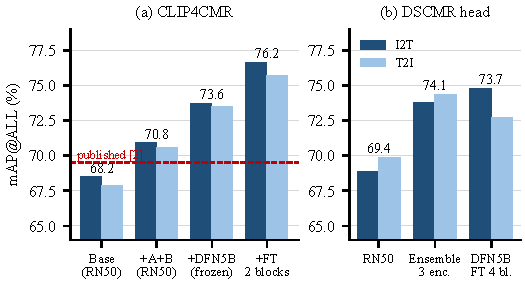
\includegraphics[width=\columnwidth]{fig_results.pdf}
\caption{Test mAP@ALL (\%, mean of 5 seeds) for (a) CLIP4CMR improvements and (b) the original DSCMR head on different input features. Numbers above bars are the average of both directions; the dashed line marks the average published result of CLIP4CMR~\cite{clip4cmr}.}
\label{fig:results}
\end{figure}

\subsection{Results for DSCMR}
Table~\ref{tab:dscmrloss} shows the loss modifications on the original DSCMR split and features. SupCon improves I2T by 1.15 points on all five seeds but does not improve T2I, and none of the tuned variants exceeds the default-weight baseline (68.05 average over three seeds). Adaptive loss weights have almost no effect.

\begin{table}[t]
\centering
\caption{Loss modifications for DSCMR (original split, test, 5 seeds)}
\label{tab:dscmrloss}
\footnotesize
\setlength{\tabcolsep}{3pt}
\begin{tabular}{@{}lccc@{}}
\toprule
Variant (tuned weights) & I2T & T2I & Paired gain (seeds) \\
\midrule
B0*: original loss & 66.02 & 68.42 & -- \\
B1*: SupCon, $\tau = 0.2$ & 67.17 & 68.24 & +1.15 / $-$0.18 (5, 1) \\
B2*: adaptive weights & 66.52 & 68.40 & +0.50 / $-$0.02 (4, 2) \\
B3*: both & 67.06 & 68.07 & +1.04 / $-$0.35 (5, 3) \\
\bottomrule
\end{tabular}

\vspace{2pt}
\parbox{\columnwidth}{\scriptsize Reference: DSCMR with default weights reaches 66.77 / 69.32 (3 seeds).}
\end{table}

Table~\ref{tab:dscmrfeat} and Fig.~\ref{fig:results}(b) report the original DSCMR head on the CLIP4CMR split with new input features. Using caption-mean RN50 features gives a baseline of 69.38. DFN5B features raise the CV score by about four points, and the two candidate configurations are virtually tied on CV (73.04 for fine-tuning four blocks, 73.03 for the ensemble; two blocks give 72.71). Following the rule fixed before opening the test set, the fine-tuned model is the primary configuration. It improves by +4.36 on average (+5.93 / +2.81 paired, 5/5 seeds); the ensemble, reported as secondary, reaches 74.06.

\begin{table}[t]
\centering
\caption{Original DSCMR head on new features (test, 5 seeds)}
\label{tab:dscmrfeat}
\footnotesize
\setlength{\tabcolsep}{3pt}
\begin{tabular}{@{}lccc@{}}
\toprule
Input features & I2T & T2I & Avg. \\
\midrule
CLIP RN50 (baseline) & 68.86 $\pm$ 0.47 & 69.89 $\pm$ 0.28 & 69.38 \\
Ensemble of 3 (secondary) & 73.75 $\pm$ 0.33 & 74.38 $\pm$ 0.47 & 74.06 \\
\textbf{DFN5B, FT 4 blocks (primary)} & \textbf{74.78 $\pm$ 0.51} & \textbf{72.70 $\pm$ 0.62} & \textbf{73.74} \\
\bottomrule
\end{tabular}

\vspace{2pt}
\parbox{\columnwidth}{\scriptsize CLIP4CMR split; text features are the mean of the five caption embeddings.}
\end{table}

\section{Discussion}
\textbf{Sources of improvement.} For CLIP4CMR, the three groups of changes contribute similar amounts: about 2.6 points from semantic prototypes and per-caption training, 2.9 from the stronger encoder and 2.5 from fine-tuning. The control experiment is important: an adapter with random prototypes does not help and can hurt, so the gain of A comes from injecting class semantics. For DSCMR, almost the entire gain comes from better input features: strengthening its nearly inactive common-space term improved only one retrieval direction.

\textbf{Negative results.} Beyond the DSCMR loss variants, re-ranking with dual-softmax and database-side augmentation added at most 0.15 points on CV and requires access to the whole retrieval set, so it was not used. Fine-tuning more blocks did not help CLIP4CMR (4 blocks: 72.90 versus 73.24 on CV).

\textbf{Limitations.} The CLIP4CMR split comes from a third-party mirror that, although verified, has not been confirmed by the authors. The improved DSCMR is evaluated on the CLIP4CMR split and therefore cannot be compared with its published numbers on the same test set. A large part of the improvement is due to stronger pre-trained encoders and requires more computation than the original methods. All results are on a single small dataset with 200 test pairs, where differences below about one point may be noise; validation on larger benchmarks is left for future work.

\section{Conclusion}
We revisited DSCMR and CLIP4CMR under a protocol that never uses the test set for model selection. Replacing the random prototypes of CLIP4CMR with semantic prototypes from CLIP prompts, training on individual captions, using a stronger encoder and partially fine-tuning it improves mean mAP from 68.17 to 76.15 on Pascal Sentence, consistently across seeds. For DSCMR, a supervised contrastive objective helps only image-to-text retrieval, while stronger features improve it by 4.36 points. Our results suggest that evaluation protocol matters as much as the method, and that visual feature quality is the main bottleneck on this benchmark.

Code and results: \url{https://github.com/sotbatchien123/dscmr-clip4cmr-pascal}

\begin{thebibliography}{00}
\bibitem{dscmr} L. Zhen, P. Hu, X. Wang, and D. Peng, ``Deep supervised cross-modal retrieval,'' in \textit{Proc. IEEE/CVF Conf. Comput. Vis. Pattern Recognit. (CVPR)}, 2019, pp. 10394--10403.
\bibitem{clip4cmr} Z. Zeng and W. Mao, ``A comprehensive empirical study of vision-language pre-trained model for supervised cross-modal retrieval,'' arXiv:2201.02772, 2022.
\bibitem{clip} A. Radford \textit{et al.}, ``Learning transferable visual models from natural language supervision,'' in \textit{Proc. Int. Conf. Mach. Learn. (ICML)}, 2021, pp. 8748--8763.
\bibitem{pascal} C. Rashtchian, P. Young, M. Hodosh, and J. Hockenmaier, ``Collecting image annotations using Amazon's Mechanical Turk,'' in \textit{Proc. NAACL HLT Workshop Creating Speech Lang. Data Amazon's Mechanical Turk}, 2010, pp. 139--147.
\bibitem{supcon} P. Khosla \textit{et al.}, ``Supervised contrastive learning,'' in \textit{Proc. Adv. Neural Inf. Process. Syst. (NeurIPS)}, 2020.
\bibitem{dfn} A. Fang, A. M. Jose, A. Jain, L. Schmidt, A. Toshev, and V. Shankar, ``Data filtering networks,'' in \textit{Proc. Int. Conf. Learn. Represent. (ICLR)}, 2024.
\bibitem{eva02} Y. Fang, Q. Sun, X. Wang, T. Huang, X. Wang, and Y. Cao, ``EVA-02: A visual representation for neon genesis,'' arXiv:2303.11331, 2023.
\bibitem{siglip} X. Zhai, B. Mustafa, A. Kolesnikov, and L. Beyer, ``Sigmoid loss for language image pre-training,'' in \textit{Proc. IEEE/CVF Int. Conf. Comput. Vis. (ICCV)}, 2023, pp. 11975--11986.
\bibitem{checkpointing} T. Chen, B. Xu, C. Zhang, and C. Guestrin, ``Training deep nets with sublinear memory cost,'' arXiv:1604.06174, 2016.
\bibitem{clipadapter} P. Gao \textit{et al.}, ``CLIP-Adapter: Better vision-language models with feature adapters,'' \textit{Int. J. Comput. Vis.}, vol. 132, pp. 581--595, 2024.
\bibitem{vgg} K. Simonyan and A. Zisserman, ``Very deep convolutional networks for large-scale image recognition,'' in \textit{Proc. Int. Conf. Learn. Represent. (ICLR)}, 2015.
\bibitem{openclip} G. Ilharco \textit{et al.}, ``OpenCLIP,'' Zenodo, 2021, doi: 10.5281/zenodo.5143773.
\bibitem{cca} D. R. Hardoon, S. Szedmak, and J. Shawe-Taylor, ``Canonical correlation analysis: An overview with application to learning methods,'' \textit{Neural Comput.}, vol. 16, no. 12, pp. 2639--2664, 2004.
\bibitem{acmr} B. Wang, Y. Yang, X. Xu, A. Hanjalic, and H. T. Shen, ``Adversarial cross-modal retrieval,'' in \textit{Proc. ACM Int. Conf. Multimedia}, 2017, pp. 154--162.
\end{thebibliography}

\end{document}
